\documentclass[12pt,a4paper]{article}

% Pacotes básicos
\usepackage[utf8]{inputenc}     % Codificação do arquivo
\usepackage[T1]{fontenc}        % Acentos corretos
\usepackage[brazil]{babel}      % Português do Brasil
\usepackage{graphicx}           % Inclusão de imagens
\usepackage{float}              % Melhor controle de posição de figuras/tabelas
\usepackage{amsmath, amssymb}   % Símbolos matemáticos
\usepackage{hyperref}           % Links clicáveis
\usepackage{caption}            % Legendas personalizadas
\usepackage{cite}               % Gerenciamento de citações

\graphicspath{{./}{../}{../../}{../../plots/}{../../plots/img/}}
\DeclareGraphicsExtensions{.pdf,.png,.jpg,.jpeg}

\title{Relatório do Projeto de Grafos e Algoritmos de Busca}
\author{Grupo X \\ Disciplina Y \\ Universidade Z}
\date{\today}

\begin{document}

\maketitle
\tableofcontents
\newpage

\section{Introdução}
Nesta seção, deve ser apresentada uma visão geral do problema, os objetivos do relatório e uma breve descrição das tarefas realizadas. 
\cite{cormen}.

\section{Modelagem do Problema em Forma de Grafo}
O problema da \textit{Ponte e da Tocha} foi modelado como um problema de busca em espaço de estados e também como um CSP (\textit{Constraint Satisfaction Problem}). Essa abordagem permite tanto a análise formal do problema em termos de grafos, como também a aplicação de algoritmos de busca clássicos para encontrar soluções ótimas. 

A seguir, a modelagem será descrita em camadas: definição de estados, ações, função sucessora e custos.

\subsection{Estados}
Seguindo a descrição do enunciado, o estado será representado da seguinte forma:

\[
S = (\text{Left}, \text{torch})
\]

Onde:
\begin{itemize}
    \item $\text{Left} \subseteq \{A, B, C, D\}$ representa o conjunto de pessoas no lado inicial da ponte;
    \item $\text{torch} \in \{\text{início}, \text{final}\}$ indica a posição atual da tocha.
\end{itemize}

Assim, temos:
\begin{itemize}
    \item Estado inicial: $({A, B, C, D}, \text{`início'})$;
    \item Estado objetivo: $(\{\}, \text{`final'})$.
\end{itemize}

O lado \textit{final} é implicitamente definido como o complemento de $\text{Left}$.

\subsection{Ações e Função Sucessora}
Cada ação corresponde ao movimento de uma ou duas pessoas através da ponte, levando sempre a tocha consigo. A função sucessora gera todos os estados possíveis a partir de um estado atual, respeitando as regras do problema.

\begin{itemize}
    \item Se $\text{torch} = \text{início}$: escolher 1 ou 2 pessoas de $\text{Left}$ para atravessar para o final;
    \item Se $\text{torch} = \text{final}$: escolher 1 ou 2 pessoas de $\text{Right}$ (o complemento de $\text{Left}$) para retornar ao início.
\end{itemize}

O custo de cada ação é definido como o tempo da travessia, que corresponde ao tempo da pessoa mais lenta entre as selecionadas.

\subsection{Exemplos Ilustrativos de Caminhos}
Na Figura \ref{fig:cen1} é mostrado o caminho ótimo com cinco movimentos, cujo custo total é de 17 minutos. Esse caminho é considerado ótimo pois minimiza o tempo total necessário para que todas as pessoas atravessem a ponte.

\begin{figure}[H]
    \centering
    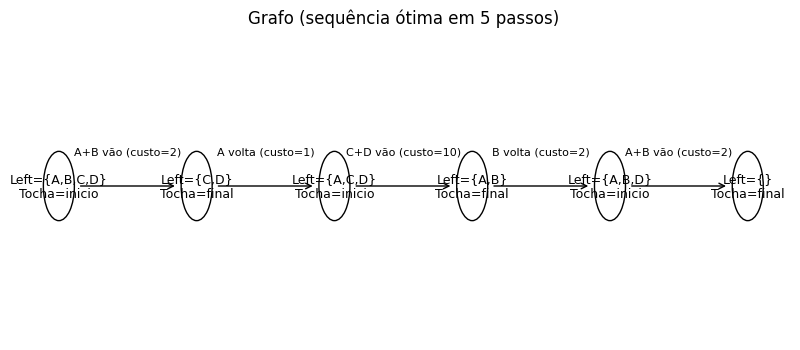
\includegraphics[width=0.8\linewidth]{optimal_path}
    \caption{Grafo ilustrando a sequência ótima em 5 passos, com movimentos de ida e volta intercalados e custo total de 17 minutos.}
    \label{fig:cen1}
\end{figure}

Na Figura \ref{fig:cen2} apresenta-se um exemplo de ramificação do grafo de estados, mostrando duas escolhas possíveis de ida (A+B ou A+C) e os estados resultantes após o retorno da tocha. Essa ilustração evidencia a multiplicidade de caminhos que podem ser explorados durante a busca.

\begin{figure}[H]
    \centering
    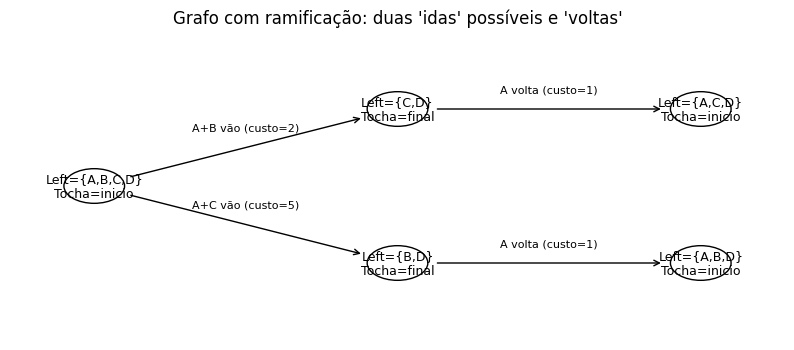
\includegraphics[width=0.8\linewidth]{ramification.png}
    \caption{Grafo com ramificação: duas possibilidades de ida e as respectivas voltas, mostrando a expansão do espaço de estados.}
    \label{fig:cen2}
\end{figure}

\subsection{Definição Formal do Grafo}
De forma resumida:
\begin{itemize}
    \item Vértices: cada vértice corresponde a um estado $S = (\text{Left}, \text{torch})$;
    \item Arestas: cada aresta representa uma ação válida (ida ou volta de 1 ou 2 pessoas), com custo associado ao tempo da travessia;
    \item Justificativa: essa modelagem é natural porque o espaço de estados é finito e discreto, permitindo a aplicação direta de algoritmos de busca como BFS e DFS;
    \item Exemplos ilustrativos: os diagramas apresentados nas Figuras \ref{fig:cen1} e \ref{fig:cen2} ajudam a visualizar as transições de estados.
\end{itemize}

\section{Rotinas Desenvolvidas}
Explicar detalhadamente as rotinas implementadas.
\begin{itemize}
\item Estrutura geral do código;
\item Funções principais;
\item Decisões de implementação.
\end{itemize}

\section{Algoritmos de Busca Estudados}
Apresentar uma explicação básica dos algoritmos analisados.
\begin{itemize}
\item Busca em Largura (BFS);
\item Busca em Profundidade (DFS);
\item Outros algoritmos relevantes (caso aplicável).
\end{itemize}

\section{Comparação e Discussão dos Resultados}
Comparar os algoritmos aplicados para solucionar o puzzle.
\begin{itemize}
\item Critérios de comparação (tempo de execução, número de passos, consumo de memória, etc.);
\item Tabelas e gráficos com resultados;
\item Discussão dos pontos fortes e fracos de cada abordagem.
\end{itemize}

\section{Conclusão}
Apresentar as conclusões gerais do trabalho, destacando os principais aprendizados e possíveis melhorias futuras.

\section*{Referências}
\bibliographystyle{plain}
\bibliography{references}

\end{document}
